% Copyright (c) 2019-2020  Zubax Robotics  <info@zubax.com>
%
% Distributed under BY-NC-ND (attribution required, non-commercial use only, no derivatives).
%

\documentclass{zubaxdoc}
\graphicspath{{../document_templates/documentation_template_latex/}{figures/}}
\title{Zubax Komar Datasheet}

\hbadness=10000

\begin{document}
\frontmatter
\begin{titlepage}

\section*{Overview}

Zubax Komar is a high-quality FOC ESC based on the \text{T\'elega} motor control technology. Komar is designed for
use in propulsion systems of light unmanned aerial vehicles (UAV), unmanned underwater vehicles (UUVs) and
unmanned surface vehicles (USVs). State-of-the-art vector control algorithms make Komar one of the most
energy-efficient ESCs on the market. Komar is compatible with almost all PMSM and BLDC motors and measures
the motor parameters to continually optimize itself for best performance. Komar is based on the Mitochondrik
control module, the hardware design of which is open source and available on
Github.\footnote{\url{https://github.com/Zubax/Komar}}

\section*{Features}

\begin{itemize}[leftmargin=!,labelindent=!,itemindent=0pt]
    \item Up to 2500\,W of continuous power output
    \item 13 -- 51\,V input voltage range (4 -- 12S $\text{LiCoO}_\text{2}$ battery)
    \item A software-controllable 5\,V, 0.5\,A BEC
    \item Highly energy efficient thanks to the embedded sensorless FOC algorithms
    \item Self-diagnostics and health status reporting
    \item Built-in motor temperature sensor for enhanced self-diagnostics
    \item Highly configurable (all parameters are tunable)
    \item Embedded bootloader (firmware can be updated via the CAN and USB interfaces in the field)
    \item Regenerative braking and active freewheeling
    \item No soldering required for installation or use
    \item Low noise and highly efficient courtesy of the sinusoidal motor currents and high-frequency PWM
    \item A rich set of communication interfaces
     \begin{itemize}[label=--,itemindent=0pt]
        \item CAN bus interface
        \begin{itemize}[label=*,leftmargin=8pt,itemindent=0pt]
            \item UAVCAN and Dronecode Autopilot Connector Standard-compatible connectors
            \item A doubly-redundant CAN bus interface for mission-critical applications
        \end{itemize}
        \item USB Micro-B interface for control, management, and telemetry (driverless compatibility
              with GNU/Linux, Windows, Mac OS X)
        \item Industry-standard RC PWM input
    \end{itemize}
\end{itemize}

\centering
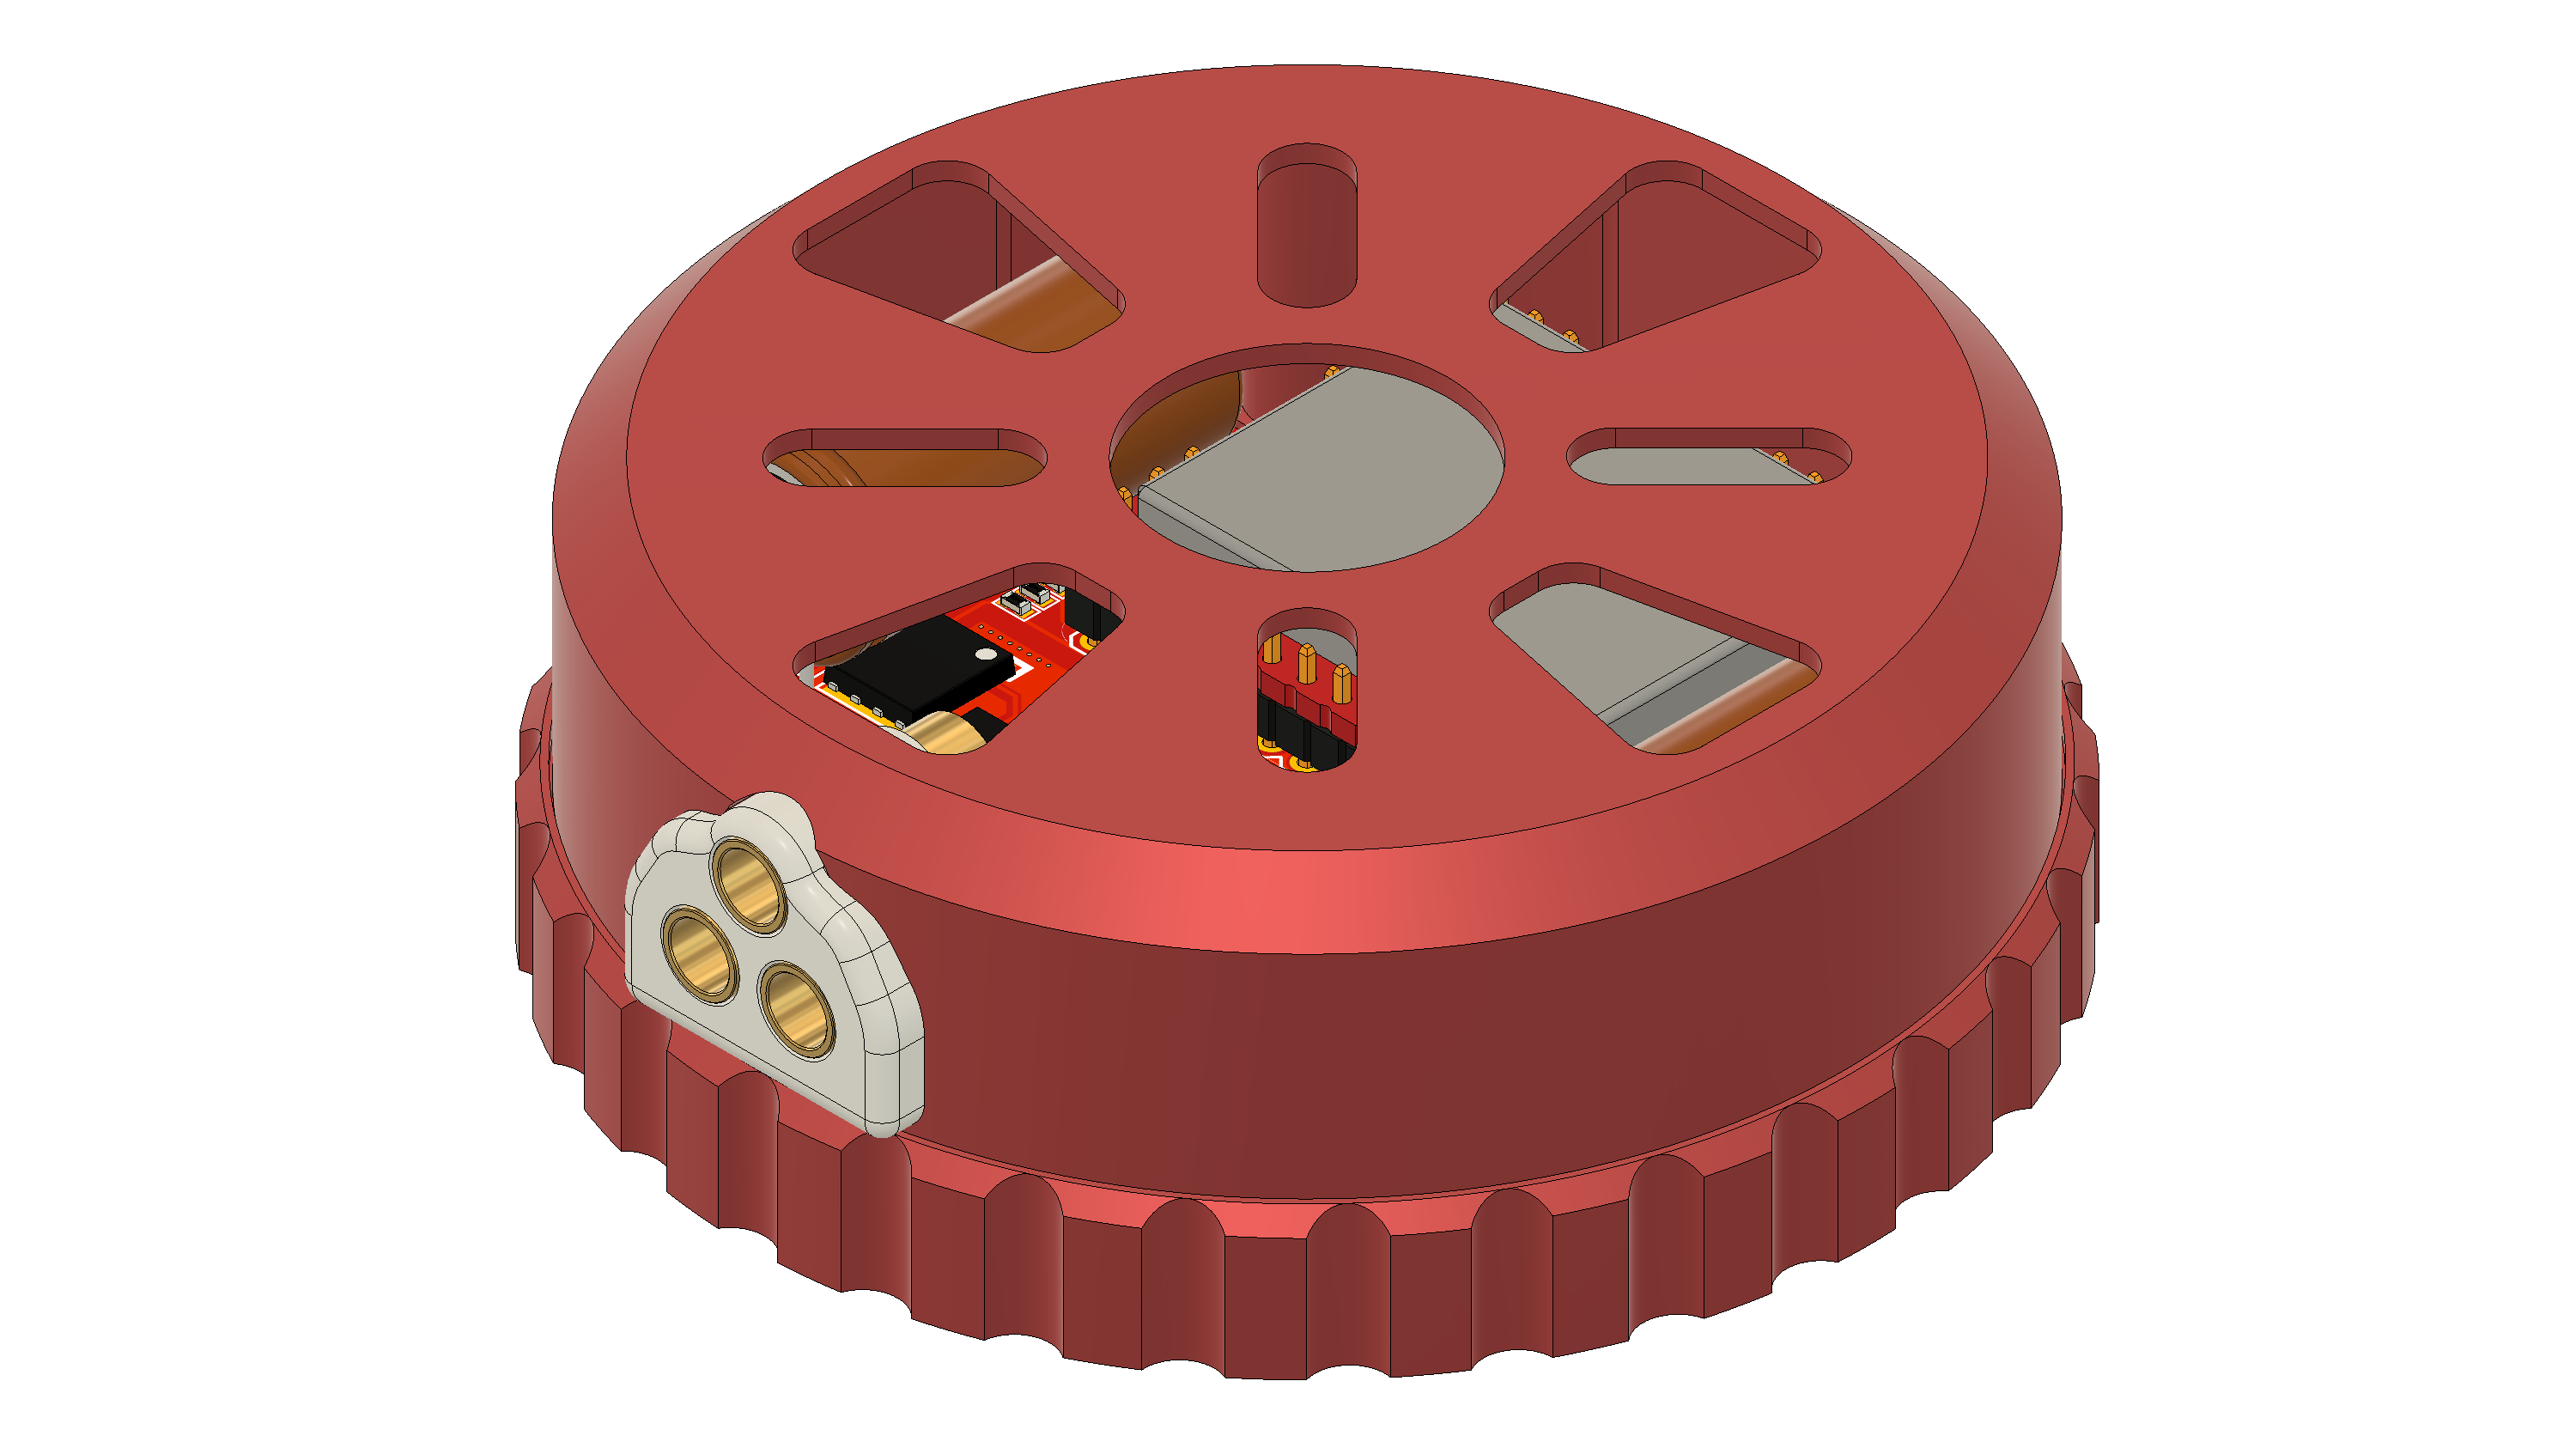
\includegraphics[width=0.6\textwidth]{top_view.png}
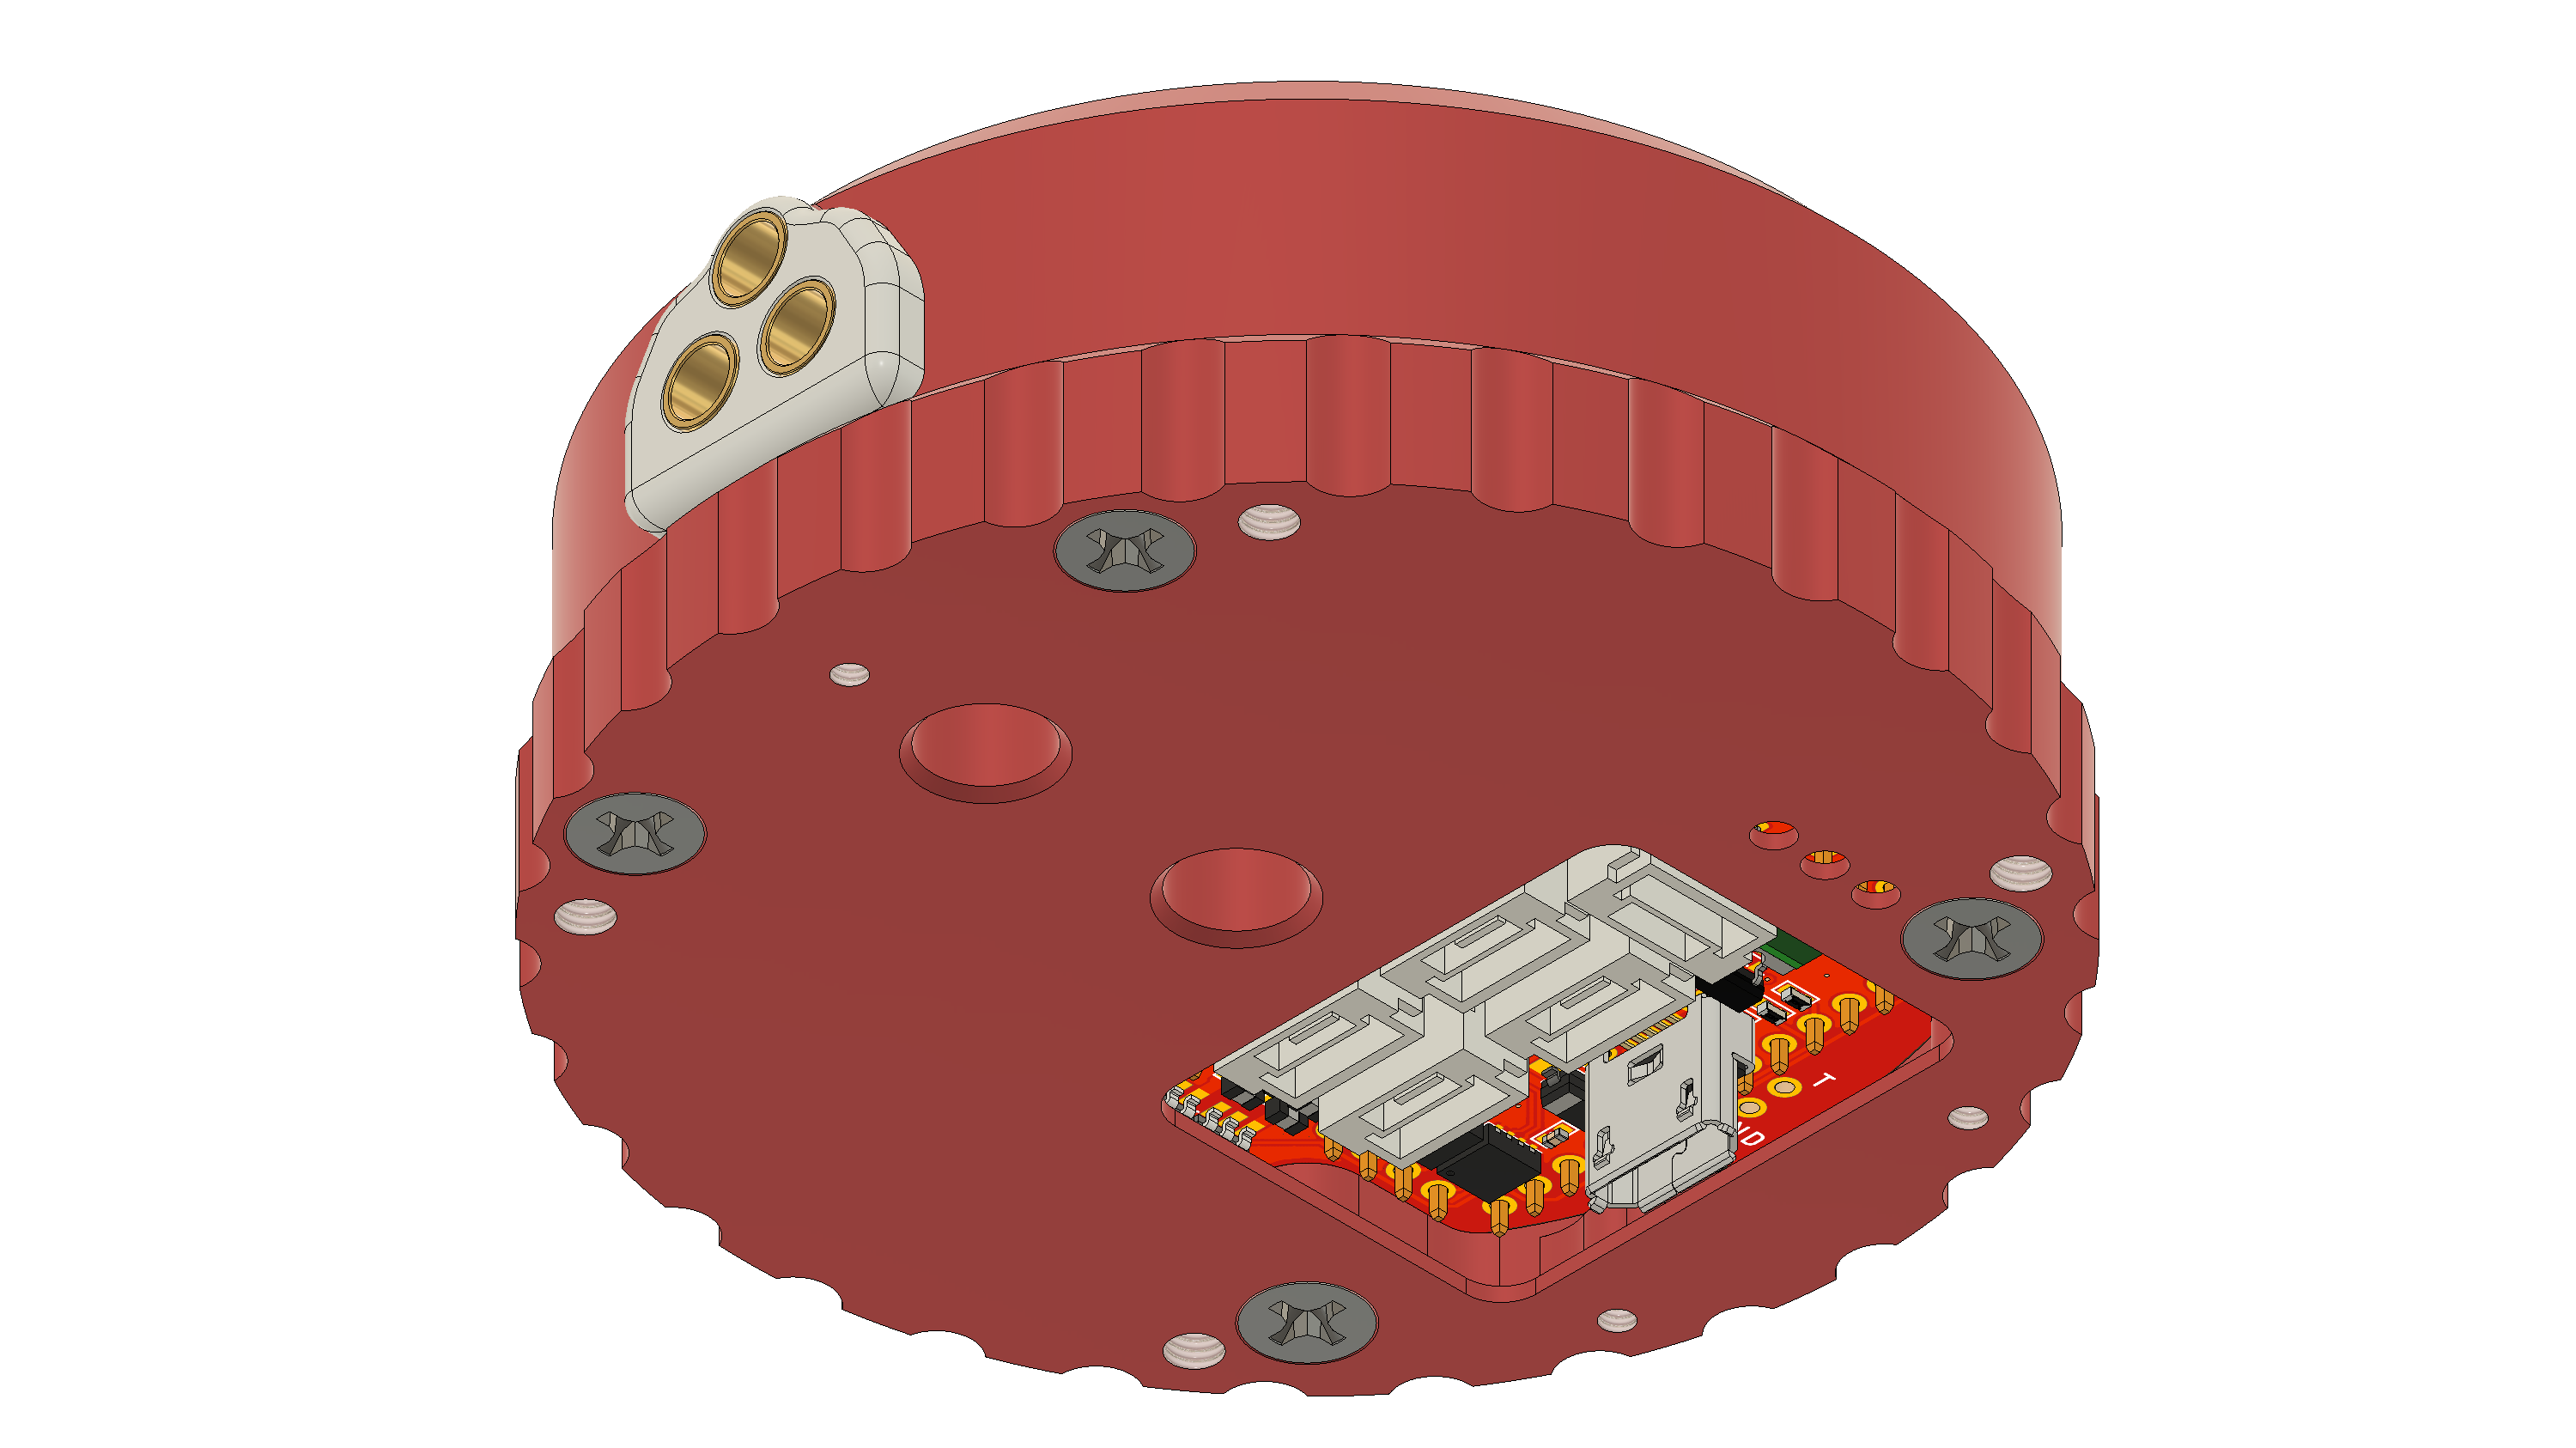
\includegraphics[width=0.6\textwidth]{bottom_view.png}

\section*{Applications}

\begin{itemize}
    \item Propeller drives for multirotor UAVs
    \item Pump and propeller drives for UUVs and USVs
    \item Fuel pump drives for jet engines and gas turbines
    \item CMG drives for LEO spacecraft
\end{itemize}

\end{titlepage}

\tableofcontents
\BeginRightColumn
\listoffigures
\listoftables

\mainmatter

\chapter{Overview}

Zubax Komar is a high-quality FOC ESC based on the Telega motor control technology. Komar is designed 
to support the propulsion systems of light unmanned aerial vehicles (UAVs), unmanned underwater vehicles (UUVs)
and unmanned surface vehicles (USVs).

The controller provides up to 2500\,W of continuous power output\footnote{When forced air cooling is applied} and
supports a wide range of operating voltages: 13 -- 51\,V (4 -- 12S $\text{LiCoO}_\text{2}$ battery).
Komar is capable of being finely tuned to any motor-propellor combination for optimal dynamic responses.

Komar offers several control modes that make it suitable for a wide range of propulsion systems.
It is fully UAVCAN-compatible and can be easily integrated into an end system using the two standard UAVCAN
Micro connectors\footnote{For more details refer to \url{https://uavcan.org/specification}} on each CAN
interface.

Ensuring high levels of system reliability, Komar continuously measures and reports on all the critical
performance parameters including the controller temperature, the motor temperature, the instantaneous
DC link voltage and instantaneous DC link current.

For further information on tuning the device and its operations, please refer to the Telega reference manual.

\section{System integration}
Zubax Komar is a single-supply device that dedicates power to the motor. It does not expose any power supply
inputs to its internal components and the 5\,V rails of the CAN interfaces cannot be used by the controller
itself. Komar does, however, offer a power delivery feature that when enabled will deliver 5\,V to the power
distribution network.

\begin{figure}[h]
    \centering
    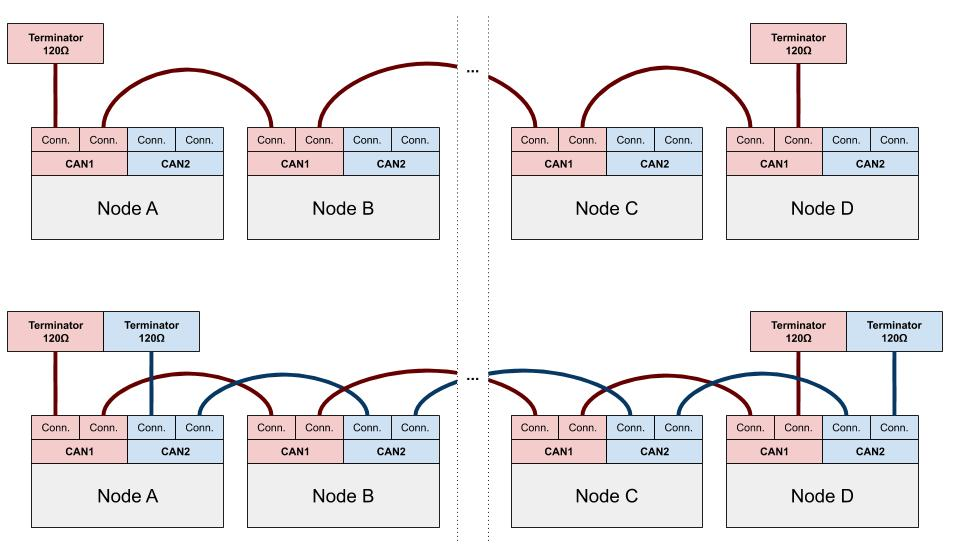
\includegraphics[width=1\textwidth]{can_integration.jpg}
    \caption{Connection of CAN nodes}
\end{figure}

\chapter{Characteristics}

\section{Absolute maximum ratings}

{\bf Warning}: Stresses that exceed the limits specified in this section may cause permanent damage to the device.

\begin{ZubaxTableWrapper}{Absolute maximum ratings}
    \begin{ZubaxWrappedTable}{| X | c  c | c |}
    Parameter                 & Min   & Max             & Unit           \\
    Supply voltage            & -0.3  & 56              &   V            \\
    Phase current amplitude   &       & 100\tnote{a}    &   A            \\
    DC continuous current     &       & 75              &   A            \\
    Operating temperature     & -40   & 85              &   \degree{}C   \\
    UART/RC PWM input voltage & -0.3  & 7               &   V            \\
    CAN H/L input voltage     & -0.3  & 7               &   V            \\
    GPIO1 input voltage       & -0.3  & 7               &   V            \\
    GPIO2 input voltage       & -0.3  & 3.6             &   V            \\
\end{ZubaxWrappedTable}
\begin{tablenotes}
        \item [a] At 25\degree{}\,C power MOSFETs temperature
\end{tablenotes}        
\end{ZubaxTableWrapper}

\section{Environmental conditions}

\begin{ZubaxTableWrapper}{Environmental conditions}
    \begin{ZubaxWrappedTable}{| l | X | c  c | c |}
    Parameter                   & Note                       & Min & Max    & Unit          \\
    Operating temperature       &                            & -40 & 85     & \degree{}C    \\
    Storage temperature         &                            & -40 & 50     & \degree{}C    \\
    Operating humidity          & Condensation not permitted & 0   & 100    & \%RH          \\
    Operating altitude          & Above mean sea level (MSL) &     & 10     & km            \\
\end{ZubaxWrappedTable}
\end{ZubaxTableWrapper}

\section{Operational characteristics}

\begin{ZubaxTableWrapper}{Power characteristics}
    \begin{ZubaxWrappedTable}{| l | X | c |}
    Parameter               & Value   &  Unit  \\
    Max continuous power    & 2,500   & W      \\
    Peak power (30\,sec)    & 3,000   & W      \\
\end{ZubaxWrappedTable}
\end{ZubaxTableWrapper}

\begin{ZubaxTableWrapper}{Electrical characteristics}
    \begin{ZubaxWrappedTable}{| X | c  c  c | c |}
    Parameter                               & Min   & Typ   & Max   & Unit            \\
    Supply voltage                          & 13    &       & 51    & V               \\
    Idle current consumption                & 3     &       & 10    & mA              \\
    FET drain-source on-state resistance    &       & 2.15  & 2.5   & $\text{m}\Omega$\\
    Inverter temperature measurement error  & -6    &       & 6     & \degree{}C      \\
    Inverter temperature measurement range  & -55   &       & 125   & \degree{}C      \\
\end{ZubaxWrappedTable}
\end{ZubaxTableWrapper}

\begin{ZubaxTableWrapper}{BEC characteristics}
\begin{ZubaxWrappedTable}{| X | l | c |}
    Parameter            & Value   & Unit \\
    Output voltage       &  4.9    & V    \\
    Voltage tolerance    &   2     & \%   \\
    Maximum load current &  500    & mA   \\
    Voltage ripple       &  100    & m$\text{V}_\text{p-p}$\\
\end{ZubaxWrappedTable}
\end{ZubaxTableWrapper}

\begin{ZubaxTableWrapper}{CAN bus interfaces characteristics}
    \begin{ZubaxWrappedTable}{| X | c  c  c | c |}
    Parameter                                       & Min   & Typ   & Max   & Unit              \\
    Bit rate                                        & 12    &       & 1000  & Kbps              \\
    Positive-going input threshold voltage          &       & 750   & 900   & mV                \\
    Negative-going input threshold voltage          & 500   & 600   &       & mV                \\
    Differential output voltage, dominant           & 1.5   & 2.0   & 3.0   & V                 \\
    Differential output voltage, recessive          & -120  & 0     & 12    & mV                \\
    Inter-connector current pass-through            & -1    &       & 1     & A                 \\
    Connector resistance during device lifetime     &       & 30    & 50    & $\text{m}\Omega$  \\
\end{ZubaxWrappedTable}
\end{ZubaxTableWrapper}

\begin{ZubaxTableWrapper}{USB interface characteristics}
    \begin{ZubaxWrappedTable}{| X | c c | c |}
    Parameter               & Min   & Max   & Unit  \\
    Low-level voltage       & 0     & 0.3   & V     \\
    High-level voltage      & 2.8   & 3.6   & V     \\
    Vbus voltage            & 1.485 & 5.5   & V     \\
\end{ZubaxWrappedTable}
\end{ZubaxTableWrapper}

\begin{ZubaxTableWrapper}{RC PWM characteristics}
    \begin{ZubaxWrappedTable}{| X | c  c  c | c |}
    Parameter                      & Min    & Typ   & Max   & Unit              \\
    RC PWM input voltage           & -0.3   & 5     & 7     & V                 \\
    RC PWM signal period           &        & 20    &       & mS                \\
    RC PWM pull down resistance    & 15     & 20    & 25    & $\text{k}\Omega$  \\
\end{ZubaxWrappedTable}
\end{ZubaxTableWrapper}

\begin{ZubaxTableWrapper}{GPIO characteristics in output mode}
    \begin{ZubaxWrappedTable}{| X | c  c  c | c |}
    Parameter             & Min    & Max            & Unit  \\
    Output voltage high   & 2      & 3.3            & V     \\
    Output voltage low    & 0      & 0.4            & V     \\
    Max current           &        & $\pm\text{20}$ & mA    \\
\end{ZubaxWrappedTable}
\end{ZubaxTableWrapper}

\begin{ZubaxTableWrapper}{GPIO characteristics in input mode}
    \begin{ZubaxWrappedTable}{| X | c  c  c | c |}
    Parameter                   & Min    & Max      & Unit  \\
    Input low level voltage     & -0.3   & 1.075    & V     \\
    Input high level voltage    & 1.485  &          & V     \\
    GPIO1 maximum voltage       &        & 7        & V     \\
    GPIO2 maximum voltage       &        & 3.6      & V     \\
\end{ZubaxWrappedTable}
\end{ZubaxTableWrapper}

\subsection{Regenerative braking}
While braking, the device transfers energy from the motor to the power supply network in a process known
as regenerative braking. Although the batteries are generally capable of absorbing the energy recovered
from braking, it should be noted that if the power supply network resistance is high, the regenerative
energy transfer may lead to a supply voltage increase that is beyond the safe operating limits of the
controller. Laboratory power supplies, for example, may present problems as this power source does not
permit high levels of reverse current. In such cases, it is advised to install additional buffer capacitors
to store the energy during braking.

\subsection{Power connectors}
The input power is provided via 100\,mm-long 14-AWG wires. The end-user should choose an appropriate power
connection method for his or her particular application.
The motor phases are connected via the female panel-mount 3,5\,mm bullet connectors. 

\newpage


\chapter{Communication interfaces}
All the communication interfaces are available via dedicated connectors.

\begin{ZubaxTableWrapper}{Connectors types}
    \begin{ZubaxWrappedTable}{| X | X |}
    Connector name          & Connector type    \\
    CAN1 (2 connectors)     & JST BM04B-GHS     \\
    CAN2 (2 connectors)     & JST BM04B-GHS     \\
    AUX                     & JST BM04B-GHS     \\
    USB                     & USB 2.0 Micro-B   \\
\end{ZubaxWrappedTable}
\end{ZubaxTableWrapper}


\begin{figure}[!hbt]
    \centering
    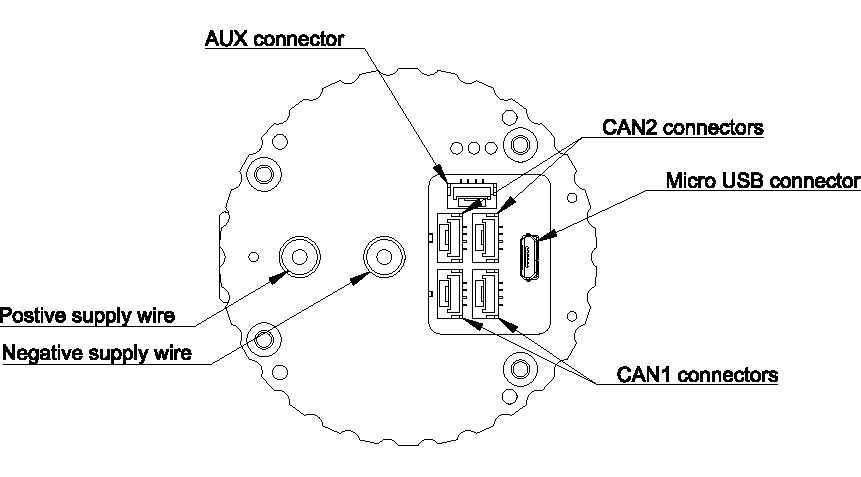
\includegraphics[width=1\textwidth]{figures/connectors_placement.pdf}
    \caption{Connectors drawing}
\end{figure}

\begin{figure}[!hbt]
    \centering
    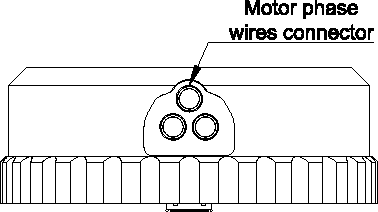
\includegraphics[width=0.5\textwidth]{figures/phase_wires.pdf}
    \caption{Motor phase wires connector drawing}
\end{figure}

\newpage

\section{CAN bus}
The device is equipped with a doubly redundant ISO 11898-2 CAN 2.0A/B interface.
Each CAN interface has two standard UAVCAN Micro connectors\footnote{Refer to \url{http://uavcan.org}
for more information on UAVCAN.} which are joined in parallel.
Please note that the CAN bus must be terminated externally since it cannot be terminated internally by
the device.

The secondary CAN bus interface (CAN2) can only be used with redundant CAN bus configurations.
With non-redundant CAN bus configurations, only the primary CAN bus connectors (CAN1) can be used; the secondary
CAN2 bus connectors should remain empty.

\begin{ZubaxSimpleTable}{CAN bus connectors pinout}{|c X X X[3]|}
	Pin no. & Type         & Name      & Comment \\
	1       & Power        & PWR       & Not internally connected to the device's circuits\\
	2       & Input/Output & CAN H     & \\
	3       & Input/Output & CAN L     & \\
	4       & Ground       & GND       & \\
\end{ZubaxSimpleTable}

\subsection{BEC output}
Zubax Komar features one software-controllable BEC output per CAN interface which can be accessed using the
bus power supply pins on the UAVCAN connectors. The BEC outputs are protected against short-circuits to
a maximum output current of 500\,mA per CAN interface. The outputs are also protected from reverse current
flows with ideal diodes. BEC outputs for both CAN interfaces are controlled by a single software parameter.

\section{USB interface}
Komar features a full-speed USB 2.0 port with a standard CDC ACM interface providing driverless compatibility
with all major operating systems (GNU/Linux, Windows, Mac OS X) and is sometimes termed the
\emph{virtual serial port}. It accepts a standard USB Micro-B connector and will report the
following properties to the USB host when connected:
\begin{itemize}
    \item Vendor ID -- 0x1D50
    \item Product ID -- 0x60C7
    \item Vendor string -- Zubax Robotics
    \item Device description string -- Zubax Robotics Telega
\end{itemize}
The USB interface uses the Popcop protocol to communicate with Kucher, the GUI software for \text{T\'elega}-based
products.

\section{GPIO}
Zubax Komar is equipped with two GPIO pins that are available on the AUX connector. While GPIO2 can only be used
for GPIO purposes, GPIO1 can be used to enable additional functions using software. These functions are: 1) the
thermistor input; and 2) the RC PWM input.

\begin{ZubaxSimpleTable}{AUX connector pinout}{|c X X X[3]|}
	Pin no. & Type         & Name      & Comment                          \\
	1       & Power        & PWR       & 5\,V power line output           \\
	2       & Input/Output & GPIO1     & RC PWM input or Thermistor input \\
	3       & Input/Output & GPIO2     &                                  \\
	4       & Ground       & GND       &                                  \\
\end{ZubaxSimpleTable}

\subsection{Thermistor input}
The PTC thermistor measures the motor windings temperature. Komar supports KTY84/130, KTY81/120 and KTY83/120
thermistors and no additional components are needed to connect the thermistor. The thermistor model can be
configured in the firmware. The thermistor should be connected between the GPIO1 and GROUND pins of the AUX
connector.

Note that most commercially-available BLDC motors do not have an embedded temperature sensor and therefore
require the end-user to install one. This is a relatively simple procedure that involves: 1) soldering
extension wires to the thermistor; and 2) gluing the thermistor to the motor winding with epoxy resin.

\subsection{RC PWM input}
Zubax Komar also supports the older analog RC PWM interface. Although this may be slow and prone
to electromagnetic interference, it remains one of the most widely-used ESC interfaces in the industry.

The RC PWM input should be connected to the GPIO1 pin of the AUX connector and then configured in the firmware.
\text{T\'elega} firmware is highly configurable when using the RC PWM interface. For a detailed description,
please refer to the \text{T\'elega} reference manual.


\chapter{LED Indication}

\newcommand{\LEDX}{{\rule{0.4em}{1.0em}}}
\newcommand{\LEDO}{{\rule{0.4em}{0.1em}}}

\newcommand{\ShowColor}[1]{{\color{#1}\rule{2em}{0.8em}}}

The device is equipped with five separate LED indicators that reflect either hardware or software status. 
Positions of LEDs on the board are shown on the figure \ref{fig:characteristics_leds_placement}.

\begin{itemize}
    \item \textbf{CAN1 and CAN2} green LEDs indicate data transfer through the CAN1 and CAN2 buses. 
           Blinks once if at least one CAN frame was successfully transmitted or successfully received in the last 
           25~ milliseconds. Glows steadily when the intensity of CAN traffic is higher than 40 frames per second.

    \item \textbf{ENABLE} orange LED indicates if the power transistor driver scheme is enabled.

    \item \textbf{GAIN} orange LED indicates the gain of motor currents measurement scheme. 
           If GAIN LED is ON, the gain is high for more accurate measurement at low power. 
           If GAIN LED is OFF, the gain is low  maintaining motor phase currents in measurement range. 
           Gain is switching automatically by firmware.

    \item \textbf{STATUS} RGB LED indicates the status of the firmware. 
          The behavior of the status LED is more complex than the other LEDs. 
          It is specified in the tables \ref{table:characteristics_status_led} 
          and \ref{table:characteristics_status_led_behavior}.
\end{itemize}

\begin{ZubaxSimpleTable}{Status LED during boot\label{table:characteristics_status_led}}{|l l X|}
    Color                     & Status                  & Description \\
    \ShowColor{yellow} Yellow & No application to boot  & The firmware haven't been 
    flashed to the ESC or FLASH has been damaged. \\
    \ShowColor{blue} Blue & Application upgrade is in progress. &   \\
    \ShowColor{green} Green & Boot canceled & The device firmware has not been properly signed. \\
    \ShowColor{magenta} Magenta   & Ready to boot & Glows after power up or restart the device 
    until the application starts.\\
\end{ZubaxSimpleTable}

\begin{ZubaxSimpleTable}{Status LED behavior\label{table:characteristics_status_led_behavior}}{|l X X|}
    LED pattern (step 80 ms) & Status & Description\\

    {\color{blue}
       \LEDX\LEDO\LEDO\LEDO\LEDO\LEDX} & Idle, ready to run & The ESC is ready and waiting for the setpoint.\\
    
    {\color{red}
       \LEDX\LEDO\LEDO\LEDO\LEDO\LEDX\LEDX\LEDX} & Idle, Hardware fault & The power stage is not ready or 
       current is tripped.\\

    {\color{red}
       \LEDX\LEDO\LEDO\LEDO\LEDO\LEDX\LEDO\LEDX\LEDX\LEDX} & Idle, Hardware test fault & The motor 
       is not connected or there is a short circuit on the output of the ESC.\\

    {\color{red}
       \LEDX\LEDO\LEDO\LEDO\LEDO\LEDX\LEDO\LEDX\LEDO\LEDX\LEDO\LEDX\LEDO\LEDX\LEDO\LEDX\LEDO\LEDX
       \LEDX\LEDX\LEDO\LEDX\LEDX\LEDX} & Idle, Invalid motor parameters & Some motor parameters 
       are not properly initialized or the motor identification hasn't been performed.\\
\end{ZubaxSimpleTable}


\chapter{Mechanical characteristics}

\begin{ZubaxSimpleTable}{Mechanical characteristics}{| l | c | X | c |}
     Parameter     & Value  & Note & Unit                     \\
     Mass          & 96.5   & Cables not included        & g  \\
     IP protection & IP54   & Liquid damage protection 
                              is achieved by conformal 
                              \mbox{coating} of the PCB  &    \\
\end{ZubaxSimpleTable}

\section{Zubax Komar drawing}
All units are in mm
\begin{figure}[!hbt]
    \centering
    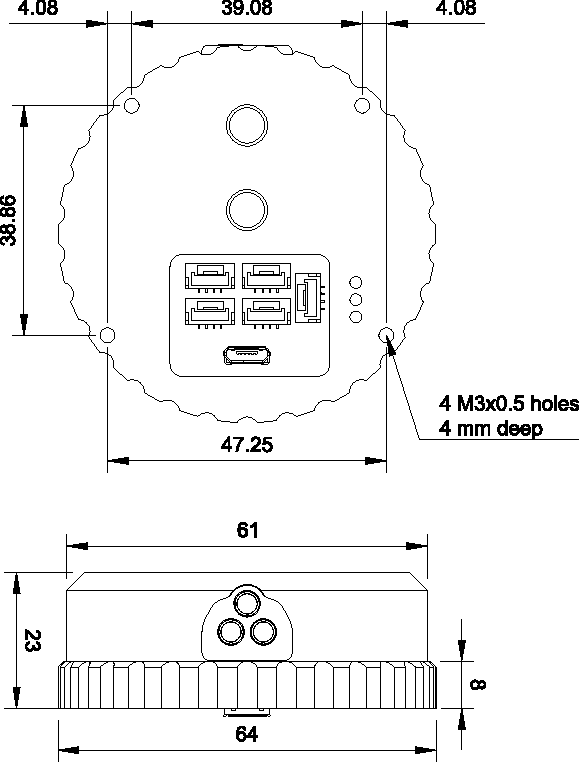
\includegraphics[width=0.7\textwidth]{mechanical_drawing.pdf}
    \caption{Zubax Komar drawing}
\end{figure}
\chapter{Motor selection considerations}
One non-obvious matter that differs FOC-enabled motor controllers (like Zubax Komar)
from conventional controllers with trapezoidal or six step commutation 
is so called voltage utilization factor.
Every BLDC motor has a characteristic that defines its theoretical maximum rotational speed. 
It is called  motor speed constant K\textsubscript{v}. 
It is measured in revolutions per minute (RPM) per volt or radians per volt second [rad/(V*s)].
Physical meaning of this constant is the number of revolutions per minute (rpm) that a motor turns when 1V (one volt) 
is applied with no load attached to that motor. 

FOC-enabled motor controllers have additional voltage utilization factor that decreases the maximum RPM 
for a given motor and supply voltage. For Komar this factor is:

\[F\textsubscript{util} = \frac{0.91}{\sqrt{3}}\]
\[RPM\textsubscript{max} = K\textsubscript{v} \times V\textsubscript{supply} \times F\textsubscript{util}\]

RPM\textsubscript{max} of a FOC enabled motor controller will always be lower than RPM\textsubscript{max} 
of a conventional controller with trapezoidal or six step commutation. This should be taken into account 
when designing a propulsion system.

For example, a motor with speed constant K\textsubscript{v} = 320 controlled by Komar running on fully charged 10S $\text{LiCoO}_\text{2}$ battery will have the following theoretical maximum RPM:

\[RPM\textsubscript{max} = 320 \times 10 \times 4.2 \times \frac{0.91}{\sqrt{3}} = 7061\]
\end{document}
